\begin{abstract}
Editing the action context of an autoregressive vision--language--action model (VLA) can change its later decoded actions, its executed motion, and its task success by very different amounts. We measure these levels separately, using context interventions that leave already emitted actions unchanged, with model-specific no-op and replay checks. In AutoVLA driving plans, replacing a ground-truth latest motion token with a frozen model token increases severe open-loop trajectory events by 25.5 percentage points (pp) in 100 failure-selected scenes, also behind a natural older token; repeated-correction effects recur on new drives, and design-weighted eligible-frame effects are about 4\,pp. In VLA-0, which emits actions as integer text, editing the action vector immediately before the continuation changes the continuation more than editing the vector before it (normalized difference 0.0137, 95\% task-cluster interval $[0.0115,0.0157]$; 149 observations, 30 LIBERO tasks). In paired rollouts through VLA-0's official ensemble loop, such context-only edits first change the executed command three steps after the first edited call and change end-effector paths by 0.8--9.2\,mm after 48 steps in four task--state units. SpatialVLA rollouts show physical deviations while task-equal success effects are bounded only within $\pm10$\,pp. AutoVLA and VLA-0 share a Qwen2.5-VL-3B backbone. In SpatialVLA (SigLIP/Gemma~2), a verified within-call path with pre-registered distance-matched donors again yields a larger response to the latest than to the older preceding action (normalized difference 0.048, 95\% layout-bootstrap interval $[0.026,0.072]$; 69 observations, 34 layouts, two SimplerEnv tasks). The pattern is thus observed in a second backbone family, without isolating a backbone effect.
\end{abstract}

\section{Introduction}
Autoregressive VLAs condition later actions on earlier generated tokens. This dependence supports coherent plans, but an inaccurate prefix can also change later predictions. Driving and manipulation policies use different action representations and generation orders: AutoVLA emits discrete motion codes~\cite{zhou2025autovla}, VLA-0 writes action vectors as integer text~\cite{goyal2025vla0}, and OpenVLA and SpatialVLA use binned or spatial action tokens~\cite{kim2024openvla,qu2025spatialvla}. A visible response to an action-token intervention establishes sensitivity to that intervention. Whether it also changes what is executed, how the system moves, and whether the task succeeds are separate empirical questions.

We therefore measure an intervention at three levels: (i) the \emph{decoding response} of later actions to a controlled edit of earlier action context; (ii) its propagation into \emph{executed commands and physical motion}; and (iii) \emph{task outcome}. Replacing a model action with ground truth (GT) changes both its error and the information available to the decoder, a changed action can move a reconstructed endpoint even when later local actions are fixed, and changed motion need not change success. Figure~\ref{fig:cases} illustrates why neither GT-conditioned correction nor a large trajectory response is a uniform utility guarantee.

We contribute:
\begin{enumerate}[leftmargin=*,itemsep=1pt,topsep=2pt]
\item \textbf{A reproducible intervention-path procedure.} Context edits leave emitted actions fixed and use frozen token sources. In VLA-0, no-op self-patches, dtype-preserving replays through its official execution loop, and simulator determinism checks verify the path; in SpatialVLA, self-patches verify a fresh-cache evaluation path. Manifests, analysis code, and table-generation scripts accompany the paper.
\item \textbf{Position-specific decoding responses in three policies.} In AutoVLA, the latest-position contrast persists behind a natural older context value. In VLA-0 and, under pre-registered distance-matched donors, in SpatialVLA, latest-action edits produce larger continuation responses than older-action edits with the intermediate action held fixed.
\item \textbf{A staged link to motion and outcome.} AutoVLA motion controls separate plan geometry from decoder response. Paired VLA-0 rollouts measure physical propagation; SpatialVLA rollouts measure physical deviation alongside bounded two-task mean success effects.
\end{enumerate}

\section{Related Work}
\paragraph{Action dependence and compounding error.}
Sequential imitation learning distinguishes independent prediction errors from errors accumulated through visited states~\cite{ross2011dagger}. WorldVLA reports deterioration during autoregressive action generation and proposes masking prior actions~\cite{cen2025worldvla}. Action dependence and possible propagation are therefore established; we estimate controlled context contrasts and follow them into execution.

\begin{figure*}[t]
\centering
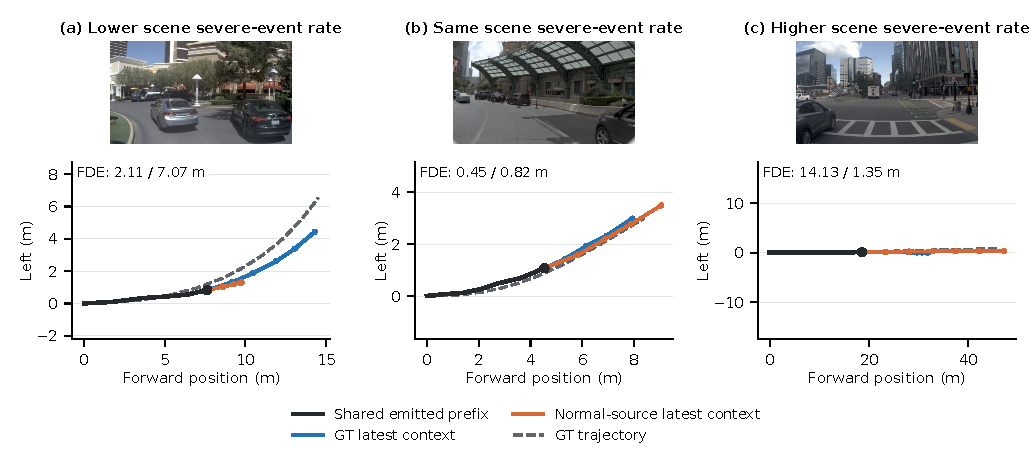
\includegraphics[width=\textwidth]{fig1_cases.pdf}
\caption{\textbf{The same latest-context correction can help or harm a generated AutoVLA plan.} Stored front-camera frames and open-loop plans from matched-prefix F. Blue uses GT at the latest context position with a natural older value (cell NAT\_REF of Fig.~\ref{fig:design}); orange uses the frozen Normal-source value there (cell NAT\_NSRC). Both share the black emitted prefix. FDE pairs are blue/orange at 5\,s. Cases are selected near group-median scene FDE differences: 87/100 scenes have a lower scene-mean severe-event rate, 12 an unchanged rate, and one a higher rate. Images show the current front view only. Axes differ across cases. Post-hoc illustrations, not representative samples or closed-loop driving results.}
\label{fig:cases}
\end{figure*}

\paragraph{Context and history in VLAs.}
Several policies add observation history or intermediate reasoning, e.g.\ amortized multi-frame context~\cite{jang2025contextvla}, value-guided candidate selection~\cite{song2025hume}, latent reasoning~\cite{bai2026laravla}, and visual foresight with motion guidance~\cite{li2026fomovla}. Token Steering edits action tokens to steer a pretrained policy~\cite{chan2026tokensteering}, and Counterfactual Memory Audit separates memory sensitivity from warranted choices and physical value~\cite{zhang2026memoryaudit}. Our target is instead the action prefix generated \emph{within one call}, with its source and placement controlled; compressed action tokenizers such as FAST~\cite{pertsch2025fast} would need a frequency-domain notion of a local edit. Astra studies trajectory attention and action queries~\cite{ma2025astra}; prompt-redirection attacks measure changes in final physical outcomes~\cite{puthumanaillam2026redirection}. These alter architectures or instructions, rather than a frozen within-call action prefix. We do not claim priority for separating sensitivity from utility.

\paragraph{Chunking and execution.}
Action chunking changes prediction and feedback frequency; recent analyses examine expressivity, compounding error, and implicit ensembling~\cite{lazzati2026chunking}. We separate decoder-context perturbations from execution dose and trace edits through an official temporal-ensembling loop.

\section{Interventions and Evidence Levels}
\label{sec:design}
\subsection{Generation context and emitted actions}
Let $j$ index generation positions within a model call and $t$ environment time. At observation $o_t$ and instruction $\ell$,
\begin{equation}
 z_{t,j}\sim p_\theta(z\mid o_t,\ell,H_{t,j}),\quad H_{t,j}=z_{t,<j}.
\end{equation}
The decoder converts tokens to an action plan; an executor applies part or all of it before the next observation. A \emph{context edit} changes $H_{t,j}$ for later positions without changing actions already emitted. Level (i) holds $o_t$ fixed. Level (ii) measures plan geometry or executed motion; closed-loop measurements at levels (ii)--(iii) allow feedback into future observations.

\subsection{AutoVLA: repeated and matched-prefix edits}
AutoVLA produces ten motion tokens at 0.5\,s spacing from its Qwen2.5-VL-3B backbone~\cite{bai2025qwen25vl}. Let $t^*$ be the first mismatch between the stored natural plan and tokenized GT. A unit is a scene and a forced token $f$ at $t^*$; paired conditions share the emitted prefix through $t^*$.

\emph{Repeated schedules.} At each eligible step, Recent-GT replaces the latest context position with GT while earlier editable positions keep the branch's own outputs (6.8 applications and 4.3 actual changes per development-F unit); Full-GT supplies GT at all editable positions. Reverse-N inserts the previous action embedding of a separate matched Normal branch into the latest position of a Full-GT context. Primary contrasts are Recent-GT minus Normal (RN) and Reverse-N minus Full-GT (RV); both use privileged GT information.

\emph{Matched-prefix factorial} (Figure~\ref{fig:design}). Normal and Full-GT source banks are generated and frozen before any cell is decoded. At anchor $a=t^*+3$, all cells emit the same Normal-source prefix through $a-1$ and generate their own suffixes from $a$. The older position $t^*+1$ holds GT or its frozen natural value ($O\in\{\GT,\NAT\}$); the latest position $a-1$ holds GT (REF), a frozen Normal-source token (NSRC), or a frozen corrected-source token (CSRC). Edited positions remain in later contexts. Define
\begin{align}
C_{\GT}&=Y(\GT,\mathrm{NSRC})-Y(\GT,\REF),\\
C_{\NAT}&=Y(\NAT,\mathrm{NSRC})-Y(\NAT,\REF),\\
I&=C_{\GT}-C_{\NAT},\\
C_{\mathrm{src}}&=Y(\GT,\mathrm{CSRC})-Y(\GT,\mathrm{NSRC}).
\end{align}
Positive $C_{\GT}$/$C_{\NAT}$ means the Normal value is more harmful than GT. $I$ is a difference of effects, not a test of positional independence; $C_{\mathrm{src}}$ changes value and source together.

\begin{figure*}[t]
\centering
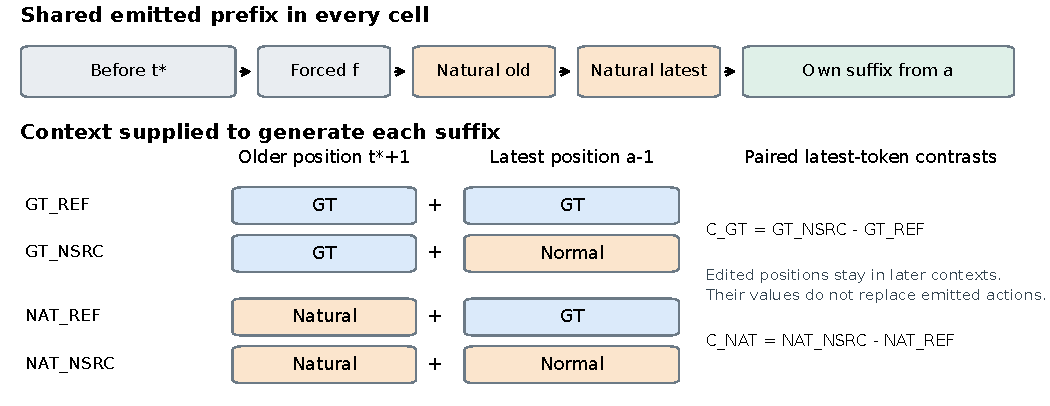
\includegraphics[width=\textwidth]{fig2_design.pdf}
\caption{\textbf{AutoVLA matched-prefix design.} Cells share all emitted pre-anchor actions; only the older ($t^*{+}1$) and latest ($a{-}1$) context positions differ, and their frozen values remain available during suffix generation. Positive $C_{\NAT}$ means the latest Normal-source value is more harmful than GT behind a natural older value. Corrected-source cells are omitted. Context edits never replace emitted actions.}
\label{fig:design}
\end{figure*}

\subsection{VLA-0: within-call action-vector edits}
VLA-0 writes eight future action vectors of seven integers (0--1000) as space-separated text~\cite{goyal2025vla0}. Its first three vectors are generated naturally and kept as the emitted prefix. We then decode the continuation (vectors 4--8) after forcing a modified copy of these three vectors into the decoder's context through the native incremental decoding path. The \emph{latest} edit (L) replaces vector 3, the \emph{older} edit (O) replaces vector 2, and OL replaces both. Donors are whole vectors from four $T{=}0.7$ samples of the same call: the first candidate whose vector differs and whose replacement keeps the token length and all tokens outside the edited span. The self-patch R forces back the natural vectors and must reproduce the natural continuation token for token. These are edits of the model's own within-call action context, not of an external observation history. The response of arm $k$ is
\begin{equation}
D(X,Y)=\frac{\sum_{\tau=4}^{8}\sum_{d=1}^{6}|s_{X,\tau d}-s_{Y,\tau d}|}{30\cdot1000},\quad A_k=D(k,R),
\end{equation}
a normalized integer-bin distance over the six arm dimensions; it is not a control command or a distance in meters.

\subsection{SpatialVLA: within-call action edits}
SpatialVLA-4B~\cite{qu2025spatialvla} emits four actions of three spatial tokens (translation, rotation, gripper) per call. The first two actions are kept as the emitted prefix. The continuation $a_3,a_4$ is decoded after forcing a conditioning copy in which $a_2$ (latest, L) or $a_1$ (older, O) is replaced by the same action of a $T{=}0.7$ sample with the natural gripper token; OL replaces both and R forces the natural copy. The non-edited action stays natural, so O measures an older-position edit with the intermediate action fixed, not total propagation. With the same $D$ form, $E_k=D(k,R)$ is the mean absolute difference of the six normalized motion components of $a_3,a_4$ (decoded before unnormalization).

\subsection{Outcomes at each level}
\emph{Decoding response (i).} For AutoVLA, the severe trajectory event is
\begin{equation}
Y=\ind[A=0\ \land\ \mathrm{FDE}_{5s}>3\,\mathrm m],
\end{equation}
with $A$ the existing coarse longitudinal/lateral acceptance rule; it is not a collision or instability measure. For VLA-0 and SpatialVLA we use $A_L-A_O$ and $E_L-E_O$.

\emph{Motion (ii).} For AutoVLA plans, let $U_s$ and $P_s$ be unperturbed and perturbed model plans under computation setting $s$ and $U_b,P_b$ a motion-baseline pair. At horizon $h$,
\begin{equation}
E_b(h;s)=\|P_s(h)-U_s(h)\|_2-\|P_b(h)-U_b(h)\|_2 .
\end{equation}
Positive excess is a larger perturbation response, not greater GT error. For VLA-0 and SpatialVLA rollouts we measure executed commands and simulator end-effector (EE) or tool-center-point (TCP) paths of paired arms.

\emph{Task outcome (iii).} SpatialVLA success contrasts are defined in Section~\ref{sec:outcome}. After paired arms execute different actions, demonstrations are not used as ground truth.

\section{Data and Inference}
\label{sec:eval}
\begin{table*}[t]
\centering\small
\caption{\textbf{Experiments, units, and evidence levels.} Units are repeated perturbations or calls within the stated independent units; F is failure-selected; E and E4 are differently weighted eligible frames. Levels: (i) decoding response, (ii) executed motion, (iii) task outcome.}
\label{tab:cohorts}
\begin{tabularx}{\textwidth}{@{}l c >{\raggedright\arraybackslash}p{1.55in} >{\raggedright\arraybackslash}X >{\raggedright\arraybackslash}X@{}}\toprule
Experiment & Level & Scenes / units & Cluster structure & Scope\\\midrule
AutoVLA repeated, development F & i & 52 / 365 & 13 drives & Failure-selected development estimate\\
AutoVLA repeated, new drives (P1-C) & i & 353 / 2,436; F: 105 / 748 & 24 drives; 18 in F & Weighted E: 2,191 eligible scenes\\
AutoVLA matched-prefix, P1-C & i & 312 / 2,160; F: 100 / 711 & F: 18 drives, 10 day--vehicles; 6 components & Weighted E4: 1,775 eligible scenes\\
AutoVLA motion response & ii (plan) & 208 / 1,453; F: 52 / 364 & 19 drives; 13 in F & Selected mechanism set\\
VLA-0 within-call pilot & i & 149 observations & 30 LIBERO tasks & Initial observations, open loop\\
VLA-0 paired rollouts & ii & 4 task--state units $\times$ 4 arms, 48 steps & 4 units (3 suites) & Truncated closed loop\\
SpatialVLA P1-D & ii, iii & Two tasks; 4,800 rollouts & Coke: 120 states; move\_near: 10 layouts & Closed loop, task-equal success\\
SpatialVLA within-call, discovery & i & 105 obs.\ (64 with donor) & 2 tasks; 35 layouts & First joint-valid of 4 donors\\
SpatialVLA within-call, follow-up & i & 105 obs.\ (69 analyzed) & 2 tasks; 34 layouts (move\_near reused) & Pre-registered distance-matched donors\\
SpatialVLA open drawer (supp.) & i & 44 obs.\ (35 analyzed) & 1 task; 15 layouts & Same rule; recovered observations\\\bottomrule
\end{tabularx}
\end{table*}

\paragraph{AutoVLA.}
We use checkpoint \texttt{AutoVLA\_PDMS\_89}~\cite{zhou2025autovla} with a 2,048-code vocabulary on NAVSIM/OpenScene scenes derived from nuPlan~\cite{dauner2024navsim,openscene2023,caesar2021nuplan}. Results concern direct action generation: the adaptive-reasoning (chain-of-thought) branch occurred in 1 of 2,748 development scenes, which was excluded, and in 0 of 5,671 scenes of the new-drive set P1-C (64 logs from 24 drives absent from development). From 2,747 natural development scenes, the mechanism sample selects 52 rejected and 156 accepted plans matched on $t^*$. E requires a complete plan and $t^*\leq7$: all 105 failure scenes and 248 sampled accepted scenes represent 2,191 eligible scenes; the matched-prefix frame E4 additionally requires $t^*\leq4$ (Table~\ref{tab:cohorts}). Scene estimates average units within scene; F uses equal scene weights and E/E4 inverse-inclusion (H\'ajek) weights.

Zero-null tests enumerate sign flips of cluster totals, assuming independent, sign-symmetric totals~\cite{winkler2015multilevel}; Holm adjustment~\cite{holm1979simple} applies within stated families. Cluster-$t$ intervals are approximate: post-hoc simulations gave 92.8--100\% coverage for nominal 95\% intervals in finite frames but 88.6\% for new drives, so some E/E4 intervals are withheld (Supplementary Sec.~B). Drives share collection days and vehicles: P1-C matched-prefix data form six connected components of the day/vehicle graph (each fixed split alone also has six; all 147 navtest logs have five), and no eligible data disjoint in both day and vehicle were available. Exact no-op, hook, and token-identity checks gave 0 logit difference and 0 token flips; cached versus full recomputation differed by at most 0.63 logits in bf16, and every token flip satisfied the pre-fixed tolerance rule. The matched-prefix gate preceded its main run; the repeated-path gate was judged after those runs.

\paragraph{VLA-0.}
We use the released LIBERO checkpoint~\cite{goyal2025vla0,liu2023libero} with its native generation configuration. A validation set (12 observations) required native-forward equality and self-patch token identity before the pilot; the pilot uses initial observations of all 30 tasks in three suites (states 1--5; 149 of 150 analyzable). Intervals are task-cluster percentile bootstraps (10,000 resamples). Paired rollouts use VLA-0's official LIBERO loop (one-step replanning, eight-chunk temporal ensemble, frame skip 10, seed 7) on four pre-registered task--initial-state units not used before. Arms start from the same state: N (natural), R (self-patch), and L/O (edit applied at every call from call 8). The executed chunk keeps the call's natural vectors 1--3 and takes the edited continuation. The unit of inference is the task--state unit ($n=4$); steps, arms, and calls are not independent samples.

\section{Level (i): Decoding Responses}
\subsection{AutoVLA: conditional effects recur, with smaller frame-wide estimates}
Repeated correction reduces severe events by 39.8\,pp in development F and reinsertion raises them by 28.6\,pp (raw exact drive $p=2.4\times10^{-4}$). On new drives, F effects recur at $-34.2$ and $+26.8$\,pp (Figure~\ref{fig:effects}a; Holm $p=2.3\times10^{-5}$, $6.1\times10^{-5}$). Weighted E effects are $-4.1$\,pp (approximate interval $[-6.2,-2.0]$) and $+3.6$\,pp. E conditions on an early natural mismatch, and much of its correction benefit comes from initially accepted scenes, so the 34--40\,pp conditional reduction is not a natural-population gain. NAVSIM v1 non-reactive PDMS~\cite{dauner2024navsim} of the same stored plans (4\,s horizon, official scorer through an in-memory metric cache) moves in the same direction: RN $+0.072$ $[0.034,0.111]$ in F and $+0.023$ $[-0.004,0.049]$ in E (Supplementary Sec.~J gives all PDMS contrasts and a metric decomposition).

\begin{figure*}[t]
\centering
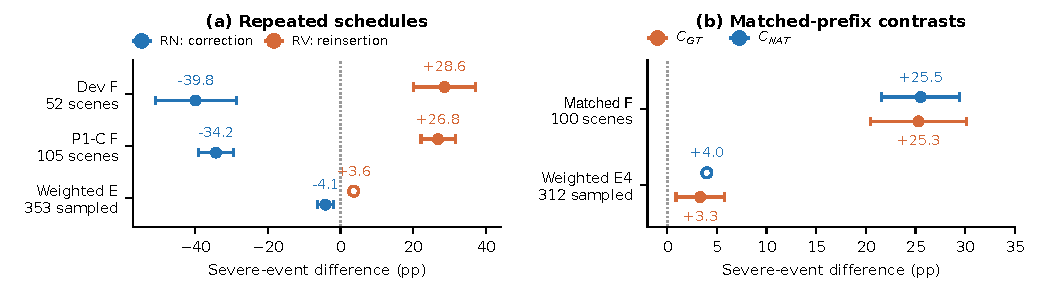
\includegraphics[width=\textwidth]{fig3_effects_relabelled.pdf}
\caption{\textbf{AutoVLA: large failure-selected effects and smaller evaluation-frame effects.} RN is Recent-GT minus Normal; RV is Reverse-N minus Full-GT; P1-C is the new-drive set; ``Matched F'' is the matched-prefix failure stratum. The matched-prefix panel changes only the latest context value within each older-context condition. Bars are approximate 95\% drive-cluster $t$ intervals retained under the interval policy (Supplementary Sec.~B); hollow points mark withheld intervals, not zero uncertainty. F, E, and E4 are different estimands.}
\label{fig:effects}
\end{figure*}

\subsection{AutoVLA: the latest-position contrast persists behind a natural older value}
The latest Normal-source token increases severe events by 25.3\,pp behind a GT older position and by 25.5\,pp behind its natural value (Figure~\ref{fig:effects}b; approximate drive intervals $[20.5,30.2]$ and $[21.6,29.4]$\,pp), with emitted pre-anchor actions and source-bank values fixed. Replacing the latest Normal value with GT lowers the scene-mean severe rate in 87 of 100 F scenes, leaves it equal in 12, and raises it in one (Figure~\ref{fig:cases}; all scene effects in Supplementary Fig.~S1). PDMS falls by 0.055 $[0.017,0.093]$ in F and 0.026 $[0.007,0.046]$ in E4 for $C_{\NAT}$. The interaction is $-0.2$\,pp ($p=0.92$; interval withheld); without a pre-specified margin, equality and irrelevance of older context are not supported. The corrected-source value reduces severe events by 15.8\,pp relative to the Normal-source value but changes value as well as source.

The F effects survive drive and day--vehicle Holm testing (Table~\ref{tab:matched}). With six components and four tests, the smallest attainable two-sided exact $p$ (0.03125) cannot pass the first Holm threshold, so no component-level rejection is possible. In E4, $C_{\NAT}=+4.0$\,pp survives drive and day--vehicle testing; $C_{\GT}=+3.3$\,pp does not survive its family threshold.

\begin{table*}[t]
\centering\small
\caption{\textbf{AutoVLA matched-prefix severe-event contrasts (pp).} Positive $C_{\GT}$/$C_{\NAT}$ is harm from substituting the frozen Normal value for GT. Each $p$ column is a separate Holm adjustment within the four-contrast family, at drive, day--vehicle, or connected-component level; family $\alpha=0.05$ for F and $0.025$ for weighted E4, pre-registered because sign-flip calibration of weighted totals showed 9--11\% type~I error at nominal 5\% (calibrated on the new-drive contrasts and inherited by the matched-prefix protocol).}
\label{tab:matched}
\setlength{\tabcolsep}{4.5pt}
\begin{tabular}{@{}lrrrrrrrr@{}}\toprule
 & \multicolumn{4}{c}{F: 100 scenes / 18 drives / 10 day--vehicles} & \multicolumn{4}{c}{E4: weighted eligible frame (312 sampled / 1,775)}\\\cmidrule(lr){2-5}\cmidrule(l){6-9}
Contrast & Estimate & Drive $p$ & Day--veh.\ $p$ & Comp.\ $p$ & Estimate & Drive $p$ & Day--veh.\ $p$ & Comp.\ $p$\\\midrule
$C_{\GT}$ & $+25.3$ & $4.6\!\times\!10^{-5}$ & 0.0078 & 0.125 & $+3.3$ & 0.051 & 0.193 & 0.375\\
$C_{\NAT}$ & $+25.5$ & $3.1\!\times\!10^{-5}$ & 0.0078 & 0.125 & $+4.0$ & $6.5\!\times\!10^{-5}$ & 0.0039 & 0.125\\
$I$ & $-0.2$ & 0.920 & 0.848 & 0.750 & $-0.7$ & 0.414 & 0.406 & 0.531\\
$C_{\mathrm{src}}$ & $-15.8$ & 0.0015 & 0.020 & 0.125 & $-2.2$ & 0.131 & 0.200 & 0.375\\\bottomrule
\end{tabular}
\end{table*}

\subsection{VLA-0: latest-vector edits have larger mean responses}
\label{sec:vla0open}
Across 149 initial observations from 30 tasks, editing the latest vector changes the continuation by $A_L=0.0297$ and the older vector by $A_O=0.0160$; the paired difference is $A_L-A_O=0.01368$ $[0.01151,0.01569]$ (Table~\ref{tab:vla0}). It persists on a source-distance-matched subset (distance ratio $0.8\leq d_L/d_O\leq1.25$; 66 observations, 27 tasks) and when the edited prefixes keep the same token set, which leaves the inherited repetition penalty's token set unchanged (79 observations; this does not rule out every logits-processor effect). The signed interaction is near zero, but the older edit still changes the response when added to the latest edit (mean $D(OL,L)=0.0152$); similar response magnitudes therefore do not imply that OL and L produce the same actions, and near-zero signed interaction does not imply additivity. Suite-level means of $A_L-A_O$ are 0.0107--0.0161 (implementation, signed-interaction definition, and validation in Supplementary Sec.~K).

\begin{table*}[t]
\centering\small
\begin{minipage}[t]{0.47\textwidth}\centering
\caption{\textbf{VLA-0 within-call responses} (normalized bins, $\times10^{-2}$; task-cluster 95\% bootstrap intervals; $^\dagger$post hoc).}
\label{tab:vla0}
\footnotesize\setlength{\tabcolsep}{2.5pt}
\begin{tabular}{@{}lrrr@{}}\toprule
Quantity & Obs./tasks & Est. & 95\% interval\\\midrule
$A_L-A_O$ (primary) & 149/30 & 1.368 & $[1.151,1.569]$\\
\ matched donor distance & 66/27 & 1.539 & $[1.198,1.900]$\\
\ same prefix token set$^\dagger$ & 79/29 & 1.486 & $[1.196,1.798]$\\
$A_L$, $A_O$ & 149/30 & 2.97, 1.60 & \\
$D(OL,L)^\dagger$ & 149/30 & 1.522 & $[1.331,1.727]$\\
signed interaction & 149/30 & $-0.113$ & $[-0.379,0.134]$\\\bottomrule
\end{tabular}
\end{minipage}\hfill
\begin{minipage}[t]{0.5\textwidth}\centering
\caption{\textbf{VLA-0 paired rollouts vs.\ N} (EE difference in mm, zero-based executed steps after the 10 settling steps; first edited call = step 8). Mean over all 48 steps / over steps 8--47. R$-$N is exactly 0 throughout.}
\label{tab:vla0cl}
\footnotesize\setlength{\tabcolsep}{2.6pt}
\begin{tabular}{@{}llccccc@{}}\toprule
Unit & Edit & 1st cmd & $>$1\,mm & Mean (48) & Mean (8--47) & Final\\\midrule
U1 & L & 11 & 15 & 2.81 & 3.37 & 4.30\\
 & O & 11 & 17 & 2.43 & 2.91 & 9.22\\
U2 & L & 11 & 18 & 1.63 & 1.96 & 3.01\\
 & O & 11 & 25 & 1.31 & 1.57 & 3.52\\
U3 & L & 11 & 28 & 1.27 & 1.52 & 5.52\\
 & O & 11 & 27 & 0.69 & 0.83 & 0.78\\
U4 & L & 11 & 17 & 2.16 & 2.59 & 5.15\\
 & O & 11 & 26 & 2.36 & 2.83 & 8.42\\\bottomrule
\end{tabular}
\end{minipage}
\end{table*}

\subsection{SpatialVLA: the latest-action pattern in a second backbone family}
\label{sec:svlares}
SpatialVLA calls use the official model and processor with a fresh generation cache per call: the library otherwise reuses a stored cache across calls, which changed 7/105 outputs after longer prompts in the first pilot (Supplementary Sec.~P). Self-patches reproduced the natural continuation tokens and EOS in every checked call (12 validation, 105 + 105 pilot, 44 drawer). A discovery pilot (first joint-valid of four donors) gave $\Delta=0.070$ $[0.044,0.100]$ over 64 observations. Its L donors were farther on average, however, and only 7 observations met its pre-specified distance matching. We therefore pre-registered a follow-up on 25 new coke layouts and the 10 reused move\_near layouts. It takes the first donor among at most 64 samples with $0.8\le d_L/d_O\le1.25$. The matched donor rule was satisfied in 69/105 observations (34 layouts), with balanced donor distances (mean $d_L$ 0.054 vs.\ $d_O$ 0.053). The primary estimate is $\Delta=0.048$ $[0.026,0.072]$, positive in both tasks (Table~\ref{tab:svla}; layout-level plots in Supplementary Fig.~S12). The latest edit changed the continuation tokens in 56/69 observations, the older edit in 27/69. $D(OL,L)=0.021$ $[0.012,0.030]$, so the older position is not irrelevant. A supplementary open-drawer task shows $\Delta=0.145$ $[0.091,0.210]$ (35 observations, 15 layouts). Responses are command-level and were not executed; the experiments are not pooled.

\begin{table}[t]
\centering\small
\caption{\textbf{SpatialVLA within-call responses} ($\Delta=E_L-E_O$, normalized action distance; 95\% layout-bootstrap intervals; separate experiments; $^{a}$one move\_near layout).}
\label{tab:svla}
\footnotesize\setlength{\tabcolsep}{2.5pt}
\begin{tabular}{@{}lrrr@{}}\toprule
Experiment (donor rule) & Obs./layouts & $\Delta$ & 95\% interval\\\midrule
Discovery, all with donor & 64/32 & 0.070 & $[0.044,0.100]$\\
Discovery, distance-matched & 7/7 & 0.084 & n/a$^{a}$\\
Follow-up, matched (primary) & 69/34 & 0.048 & $[0.026,0.072]$\\
\ coke & 55/25 & 0.042 & $[0.015,0.070]$\\
\ move\_near & 14/9 & 0.054 & $[0.018,0.093]$\\
Open drawer (supp.) & 35/15 & 0.145 & $[0.091,0.210]$\\\bottomrule
\end{tabular}
\end{table}



\section{Level (ii): Executed Commands and Motion}
\subsection{AutoVLA plans: response beyond motion extrapolation}
We perturb one context token without GT-valued replacement and compare the model's response with motion controls: coordinate accumulation (later local actions held fixed; a privileged geometry control), constant body-frame SE(2) motion (CM), zero-turn constant velocity, constant turn rate/velocity, turn rate/acceleration, and a separately trained learned non-autoregressive extrapolator, which does not isolate VLA architecture. On units observed through 2.5\,s after perturbation (Supplementary Fig.~S13), CM excess in F rises from 0.14\,m at 1\,s to 0.87\,m at 2.5\,s and accumulation excess from 0.38 to 1.82\,m; in the selected union, CM excess is only 0.01 and 0.08\,m. At the 5\,s endpoint, F excess is $+4.37$\,m $[3.35,5.20]$ over accumulation, $+2.35$ $[1.26,3.18]$ over CM, and $+1.97$ $[1.10,2.83]$ over the learned control (approximate drive-cluster bootstrap over 13 drives; coverage was not simulated for this continuous outcome). In all 208 selected scenes, CM excess is $+0.20$ $[-0.33,0.55]$\,m and learned-control excess is $-0.34$\,m (whether its interval excludes zero depends on the interval method; Supplementary Sec.~J). All six F excesses stay positive under eager-attention and fp32-arithmetic recomputation (12 tests, Holm $p\le0.0088$). Response size is not accuracy: at 2.5\,s the perturbed F plans are on average 3.04\,m from GT versus 3.76\,m for their references.



\subsection{VLA-0: context-only edits reach executed motion}
\label{sec:vla0cl}
All path checks passed (Table~\ref{tab:vla0cl}). A 16-step smoke rollout matched the native forward pass at every call. In 4 units $\times$ 4 arms $\times$ 48 steps (784 policy replans including the smoke; a replan may contain several generation calls), R reproduced N bitwise in actions, simulator states, and ensemble buffers in all four units (160/160 self-patch calls token-identical). Feeding the logged float32 chunks back through the official loop reproduced every executed action and buffer (17/17 episodes), and replaying N's actions without the model reproduced every simulator state. Arms were identical before the first edited call. The latest edit was applied at 158/160 calls (two calls lacked an eligible donor and executed the natural chunk); the older edit at 160/160 (implementation, cost, and full traces in Supplementary Sec.~L).

The first edited call is step 8; in all eight L/O comparisons the executed command and simulator state first differ at step 11. This three-step delay is what the design predicts: each call keeps its natural first three vectors, and the eight-chunk ensemble executes the step-$t$ entries of recent chunks. From step 12 on, arms observe different states, so differences include closed-loop feedback. EE paths separate by more than 1\,mm within 7--20 steps of the first edit and end 0.8--9.2\,mm apart (Table~\ref{tab:vla0cl}; traces in Supplementary Fig.~S14). The L/O ordering is mixed: the mean EE difference is larger for L in three units, the final difference larger for O in three. With four units we report this as a description, not as a population ordering, reversal, or equivalence; the open-loop $A_L>A_O$ result is not claimed to carry over to motion.





\begin{figure*}[t]
\centering
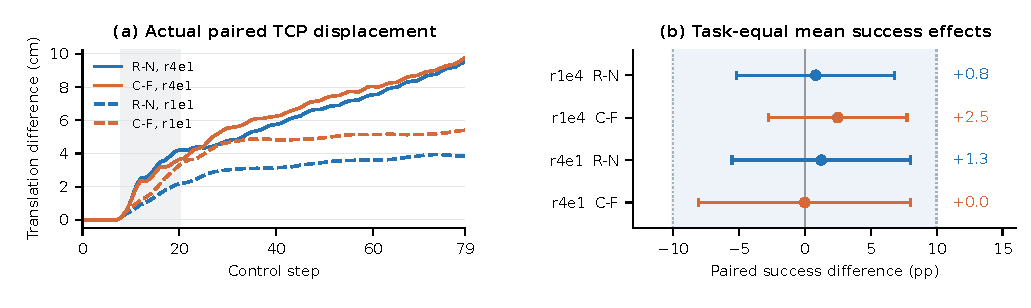
\includegraphics[width=\textwidth]{fig_spatialvla.pdf}
\caption{\textbf{SpatialVLA: physical deviation and task success are separate outcomes.} Left: mean actual TCP translation difference between paired episodes (240 units per curve); gray marks the injection span, steps 8--20; r4e1 executes four steps between replans, r1e1 replans each step. Right: task-equal success effects under r1e4 (one-step replanning, four-chunk ensemble) and r4e1, with corrected approximate 95\% intervals clustered by physical state; shading marks $\pm10$\,pp.}
\label{fig:spatial}
\end{figure*}

\subsection{SpatialVLA: physical deviation}
SpatialVLA's four-step harness crosses whether a perturbed action is executed and whether it enters context~\cite{qu2025spatialvla}: Natural (N) uses reference execution/context, Feedback (F) perturbs both, Corrected (C) executes the perturbation but restores reference context, and Reverse (R) perturbs context only. References are unperturbed policy rollouts in SimplerEnv~\cite{li2024simplerenv}, not expert GT. Context perturbations change generated actions and measured TCP paths: under r4e1 (four executed steps per replan), mean TCP deviation areas are 428 and 449\,cm$\cdot$step for $R-N$ and $C-F$ (Figure~\ref{fig:spatial}a). Under a fixed perturbation budget, r4e1-minus-r1e1 $R-N$ area is $+214$\,cm$\cdot$step (descriptive $[171,255]$); with delivered execution dose matched, the ensemble-axis interaction is $+21$ $[-25,68]$, within its original $\pm100$ margin.

\section{Level (iii): Task Outcome}
\label{sec:outcome}
For SpatialVLA, $\delta_R=S_R-S_N$ and $\delta_C=S_C-S_F$ are intervention effects on success, not natural mediation effects. Physical deviations coexist with small two-task mean success effects: under four-step replanning without ensembling (r4e1), these are $+1.3$ and $0.0$\,pp. The other success setting uses one-step replanning and four-chunk ensembling (r1e4). Corrected approximate inference (paired Newcombe intervals~\cite{newcombe1998paired} with Rao--Scott design-effect adjustment~\cite{raoscott1992clustered} and MOVER pooling~\cite{zou2008mover}) supports the original $\pm10$\,pp equivalence margin for the four two-task means but not the post-hoc $\pm5$\,pp margin (Figure~\ref{fig:spatial}b). Task-level effects are wider and are not covered by the pooled bound (Table~\ref{tab:spatial8}): r4e1 $C-F$ is $-4.2$\,pp in coke and $+4.2$\,pp in move\_near, and their cancellation does not establish task-level invariance. Coke has 120 physical initial states; move\_near reuses ten layouts across 120 units, and more seeds do not create more layouts. P1-D records successful restoration checks for 3,840 branches; 960 natural roots have no restoration field. The VLA-0 rollouts are 48-step diagnostics; their success flags are logged only and are not used to estimate success.



\begin{table}[t]
\centering\small
\caption{\textbf{SpatialVLA task-level success effects} (pp; 120 paired episodes per task and setting; approximate 95\% Newcombe intervals, design-effect adjusted for move\_near's 10 layouts). Per-task equivalence was not pre-specified and is not claimed; the $\pm10$\,pp bound concerns the two-task means.}
\label{tab:spatial8}
\setlength{\tabcolsep}{3pt}
\begin{tabular}{@{}llrrrr@{}}\toprule
Setting & Contrast & \multicolumn{2}{c}{coke} & \multicolumn{2}{c}{move\_near}\\\midrule
r1e4 & $R-N$ & $0.0$ & $[-6.5,6.5]$ & $+1.7$ & $[-8.4,11.7]$\\
 & $C-F$ & $+4.2$ & $[-2.8,11.3]$ & $+0.8$ & $[-6.9,8.6]$\\
r4e1 & $R-N$ & $+1.7$ & $[-8.3,11.6]$ & $+0.8$ & $[-8.4,10.0]$\\
 & $C-F$ & $-4.2$ & $[-14.0,5.8]$ & $+4.2$ & $[-8.6,16.7]$\\\bottomrule
\end{tabular}
\end{table}

\section{Discussion and Limitations}
\label{sec:limits}
\textbf{What the levels show.} Controlled context edits produce position-specific decoding responses in three policies with different action representations, domains, and two backbone families; the AutoVLA latest-position contrast and the direct latest-versus-older comparisons in VLA-0 and SpatialVLA are different estimands (Supplementary Sec.~S). In VLA-0 these responses reach executed commands and end-effector motion through the official loop; in SpatialVLA, physical deviation coexists with task-equal success effects bounded within $\pm10$\,pp. Decoding response, motion, and success must therefore be measured separately. The three-step VLA-0 delay verifies the intervention path rather than revealing a learned property.

\textbf{Limitations.} AutoVLA and VLA-0 share Qwen2.5-VL-3B. SpatialVLA adds a SigLIP/Gemma~2 policy, but only at the command level, on two reused simulator tasks plus one supplementary task. Observing the pattern across backbones does not isolate a backbone effect, because the policies also differ in data, action representation, and domain. Among surveyed alternatives, pi0-FAST, OpenVLA, and OpenVLA-OFT lack a time-ordered within-call channel, and WorldVLA masks it (Supplementary Sec.~T). AutoVLA results are five-second open-loop plans with GT-conditioned contrasts; they do not establish closed-loop driving failures or a deployable GT-free recovery method, and correcting toward a self-generated reference can worsen GT agreement (an earlier failure-selected analysis: $+19.7$\,pp severe events). Weighted frame effects are much smaller than failure-selected ones, and shared days and vehicles leave six components without independent day-and-vehicle validation. The VLA-0 rollouts cover four task--state units over 48 steps and do not estimate success; the pilot's observations are initial states. SpatialVLA covers two tasks with reused layouts. Impromptu VLA~\cite{chi2025impromptu} and OpenVLA analyses lack intervention-path parity evidence and remain descriptive (Supplementary Sec.~G). Several interval and visual analyses are post hoc and are labeled as such; retained-window and transient-exposure analyses of GT correction are in Supplementary Sec.~I.

\section{Conclusion}
Action-context edits in autoregressive VLAs have substantial, position-specific effects on decoded actions: in AutoVLA, latest-position matched-prefix contrasts remain large behind a natural older value, and in VLA-0 and SpatialVLA latest-action edits yield larger continuation responses than older-action edits. Verified execution replays show that such context-only edits reach executed commands and end-effector motion within a few steps, while SpatialVLA's two-task mean success effects lie within the original $\pm10$\,pp margin despite physical deviation. Measuring each level, with its own units and checks, is what makes an action-token intervention interpretable.
